\documentclass[a4paper,11pt]{article}

%%% DO NOT CHANGE %%%%%%%%%%%%
\usepackage[utf8]{inputenc}
\usepackage[T1]{fontenc}
\usepackage{lmodern}
\usepackage{amsmath,amsfonts,amssymb,epsfig,graphicx,url}

\oddsidemargin 0cm
\topmargin 0cm
\textwidth=17cm
\textheight=24cm

\thispagestyle{empty}
%%%%%%%%%%%%%%%%%%%%%%%%%%%%%%

% You may add additional languages if needed.
\usepackage[german,english]{babel}

\begin{document}

\selectlanguage{english}

%%%%%%%%%%%%%%%%%%%%%%%%%%%%%%%%%%%%%%%%%%%%%%%%%%%%%%%%%%%%%%%%%%%%
% Talk 1
\newpage

\begin{center}
\bgroup
\large
\bf
%%% Put the title here
ngsPETSc: NETGEN/NGSolve meets PETSc
\egroup
\bigskip

%%% Put the author(s) here, boldface for the presenting author
\textbf{Umberto Zerbinati}$^a$, Patrick E.~Farrell$^{a}$, and Stefano Zampini$^b$
\medskip

%%% Put affiliation(s) here
$^a$ {\em University of Oxford, United Kingdom}\\
$^b$ {\em King Abdullah University of Science and Technology, Saudi Arabia}\\
\end{center}
\bigskip

%%% Put the abstract here
\noindent
We present ngsPETSc, an interface between the NETGEN mesher \cite{netgen}, the finite element library NGSolve \cite{ngsolve} and the Portable, Extensible Toolkit for Scientific computation (PETSc) \cite{petsc}. ngsPETSc is written in Python, taking advantage of the Python bindings of Netgen/NGSolve and petsc4py \cite{petsc4py}.
The key components of ngsPETSc are the interface between NETGEN and PETSc DMPlex and the interface between NGSolve and PETSc PC, KSP and SNES.

In particular, thanks to the first component it is possible to export mesh generated from geometries described via constructive solid geometry (CSG) using OpenCASCADE as PETSc DMPlex objects.
For example, this allows Firedrake \cite{firedrake} to employ meshes described via CSG, to use higher-order meshes that conform to the geometry, and to build mesh hierarchies for geometric multigrid solvers that better approximate the domain with refinement.
This also enables the use of different mesh splits, like Alfeld and Powell--Sabin splits, which facilitate the development of conforming exactly divergence-free element pairs for incompressible flow.

Conversely, the PETSc PC, KSP, and SNES interfaces allows the use of PETSc solvers in NGSolve, giving access to a much broader range of linear and nonlinear solvers.
For example, SNES's line search features can make the solution of complex non-linear problems, like the Naghdi shell model shown in Figure \ref{fig:ngsPETSc}, much more robust.

\begin{figure}[h]
    \centering
    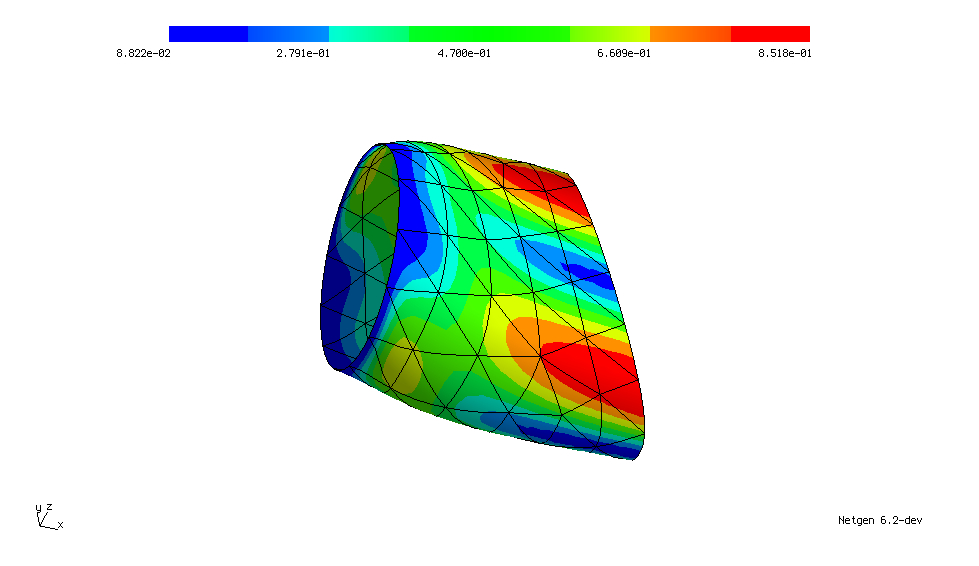
\includegraphics[width=0.75\textwidth]{../figures/naghdi.jpg}
    \caption{Naghdi shell simulation in NGSolve, solved using PETSc SNES via ngsPETSc.}
    \label{fig:ngsPETSc}
\end{figure}
Future work includes:
\begin{enumerate}
    \item the use of ngsPETSc as a linear algebra backend for NGSolve, to ensure cross-architecture compatibility, GPU support, and performance;
    \item the development of a new interface between PETSc TS and NGSolve, to solve time-dependent problems;
    \item the support for three-dimensional mesh hierarchies in Firedrake;
    \item the support for periodic meshes in Firedrake.
\end{enumerate}
%%% Put references here
\begin{thebibliography}{9.}
\frenchspacing
\bibitem{netgen}Schöberl, J., 1997. NETGEN: An advancing front 2D/3D-mesh generator based on abstract rules. Computing and visualization in science, 1(1), pp.41-52.
\bibitem{ngsolve}Schöberl, J., 2014. C++ 11 implementation of finite elements in NGSolve. Institute for analysis and scientific computing, Vienna University of Technology, 30.
\bibitem{petsc}Balay, S., Abhyankar, S., Adams, M.F., Benson, S., Brown, J., Brune, P., Buschelman, K., Constantinescu, E.M., Dalcin, L., Dener, A. and Eijkhout, V., 2023. PETSc/TAO Users Manual Revision 3.19 (No. ANL-21/39). Argonne National Lab.(ANL), Argonne, IL (United States).
\bibitem{petsc4py}Dalcin, L.D., Paz, R.R., Kler, P.A. and Cosimo, A., 2011. Parallel distributed computing using Python. Advances in Water Resources, 34(9), pp.1124-1139.
\bibitem{firedrake}Rathgeber, F., Ham, D.A., Mitchell, L., Lange, M., Luporini, F., McRae, A.T., Bercea, G.T., Markall, G.R. and Kelly, P.H., 2016. Firedrake: automating the finite element method by composing abstractions. ACM Transactions on Mathematical Software (TOMS), 43(3), pp.1-27.
\end{thebibliography}
%%%%%%%%%%%%%%%%%%%%%%%%%%%%%%%%%%%%%%%%%%%%%%%%%%%%%%%%%%%%%%%%%%%%

%%% Copy and paste the above for additional talks.

\end{document}
